The most difficult part when using a \gls{gui} is to keep track the executed functionalities during the analysis.
To face this need we equipped \gls{igro} of a \gls{rr} hidden layer (with aid of \textit{easyReporting} package) able to trace all executed code by the user.

In combination with a system of \gls{cdf}, \gls{igro} stores code chunks and the input/output data of each analysis step inside an \gls{rmd} file.

\begin{figure}
\centering
\begin{subfigure}{.5\textwidth}
  \centering
  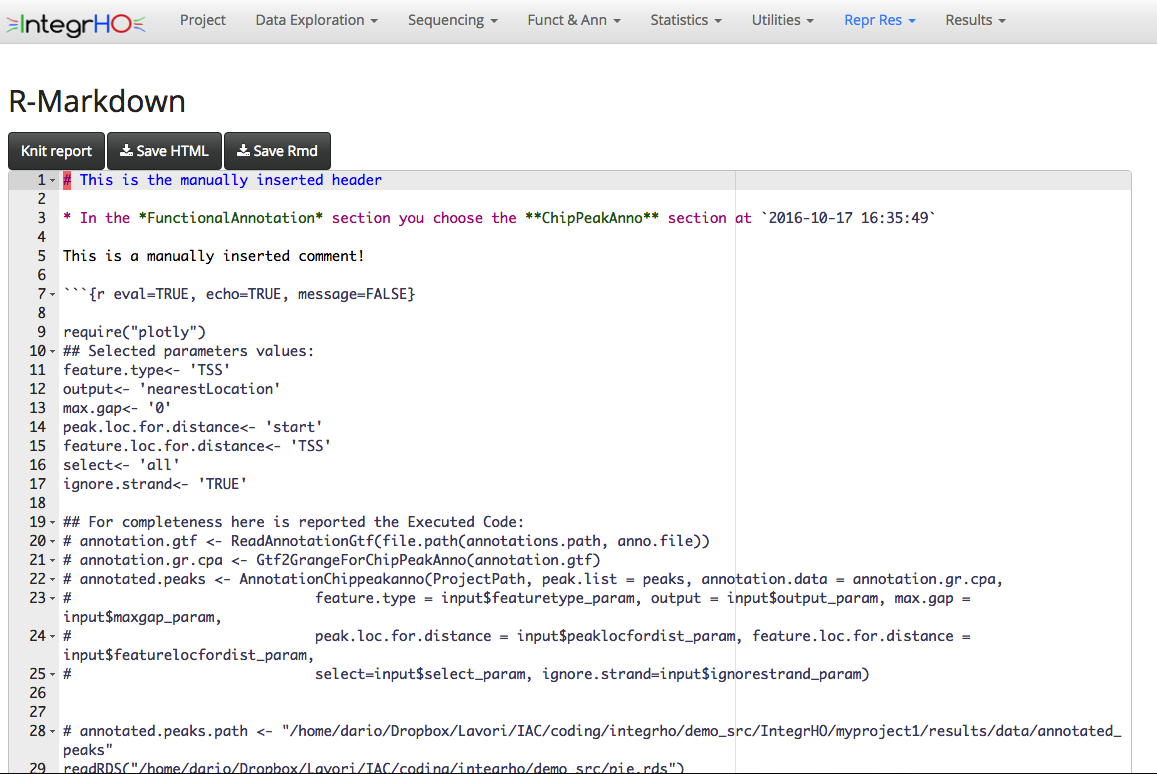
\includegraphics[width=.9\linewidth]{img/integrho/rr_1.png}
  \caption{The Interface for the editing of an auto-generated report with \gls{igro} web platform.}
  \label{fig:integrhorr1}
\end{subfigure}%
\begin{subfigure}{.5\textwidth}
  \centering
  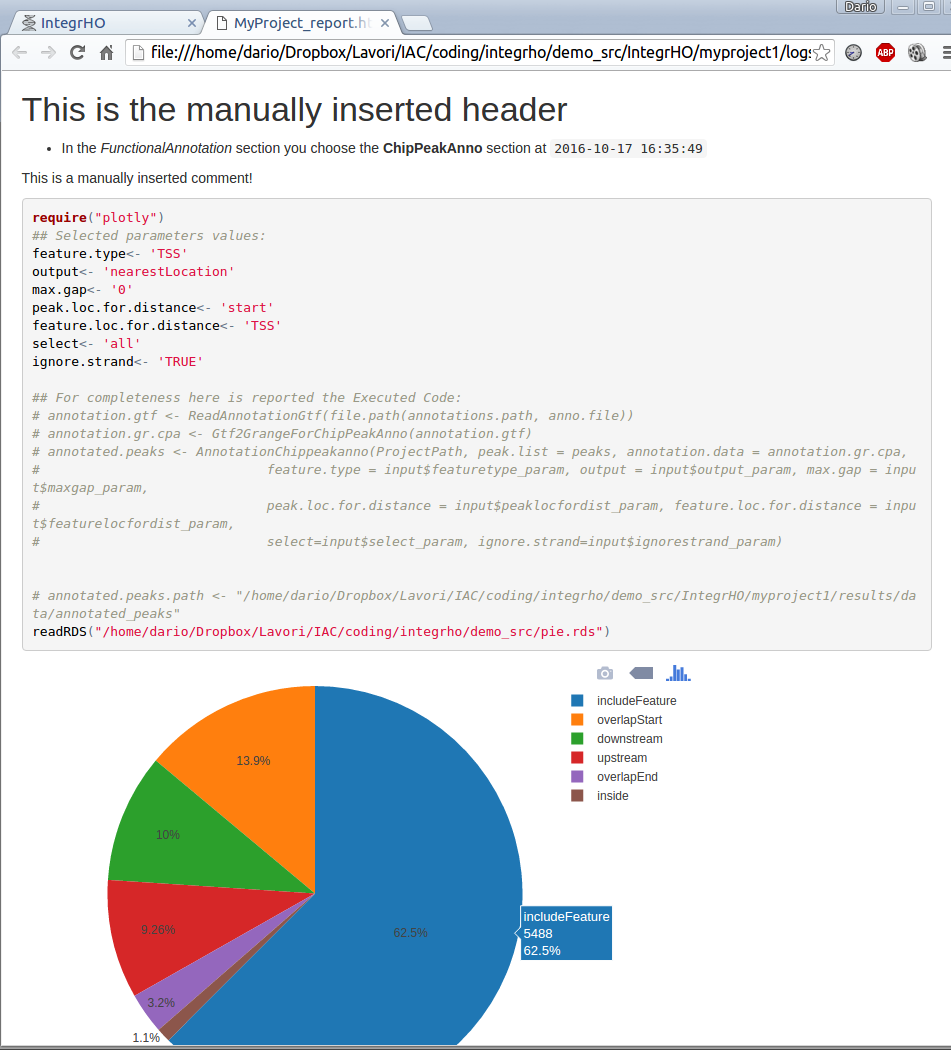
\includegraphics[width=.9\linewidth]{img/integrho/rr_2.png}
  \caption{The report compiled and enriched with manually inserted comments.}
  \label{fig:integrhorr2}
\end{subfigure}
\caption[\gls{igro} report editing]{The reproducible research with \gls{igro}.}
\label{fig:integrhorr}
\end{figure}

The auto-produced \gls{rmd} file as it is, it's not useful to show to third-parties, it needs to be enriched with natural language comments,  that's why we built a specific interface enabling the user to edit the automatically produced \gls{rmd} file and to compile it on the fly (see sub-figure \ref{fig:integrhorr1}).

The enriched output report can be produced in \gls{html} (sub-figure \ref{fig:integrhorr2}) or \gls{pdf} formats, in order to be easily attached as supplementary material of a published article, facilitating the reproducibility of the analysis to a third party user.

Furthermore, thanks to the \gls{cdf} system, each code chunk is not dependent from on previous ones, enabling the final user to add/remove code chunks.